\id{МРНТИ 65.43.31}

{\bfseries БИДАЙДЫҢ ОТАНДЫҚ СҰРЫПТАРЫН ҚОЛДАНА ОТЫРЫП СЫРА ТЕХНОЛОГИЯСЫН
ЖАСАУ}

\hl{}

{\bfseries \textsuperscript{1}Д. Н. Бақытжан}
\begin{figure}[H]
	\centering
	
\includegraphics[width=0.8\textwidth]{media/pish3/image1}
	\caption*{}
\end{figure}

{\bfseries , \textsuperscript{2}Э.Б. Аскарбеков}
\begin{figure}[H]
	\centering
	
\includegraphics[width=0.8\textwidth]{media/pish3/image1}
	\caption*{}
\end{figure}

\textsuperscript{1}Г.И.} {\bfseries Байгазиева}
\begin{figure}[H]
	\centering
	
\includegraphics[width=0.8\textwidth]{media/pish3/image1}
	\caption*{}
\end{figure}

\textsuperscript{1}А. К.
\begin{figure}[H]
	\centering
	
\includegraphics[width=0.8\textwidth]{media/pish3/image1}
	\caption*{}
\end{figure}


\emph{\textsuperscript{1}Алматы технологиялық университеті, Алматы,
Қазақстан}

\emph{\textsuperscript{2}Қазақ технология және бизнес университеті,
Астана, Қазақстан}

{\bfseries \textsuperscript{\envelope }}Корреспондент-автор: Erik\_ab82@mail.ru

\hl{}

Қазіргі уақытта Қазақстанның сыра қайнату саласы тамақ өнеркәсібін
дамытудың бәсекеге қабілетті бағыттарының бірі болып табылады.
Ассортиментті кеңейту, инновациялық технологияларды қолдану сыраның жаңа
түрлерін алуға мүмкіндік береді. Арпа уытының бір бөлігін басқа шикізат
түрлерімен алмастыру, отандық селекциядағы сыра өндіруге жарамды арпа
сұрыптарының жетіспеушілігі мәселесін шешуге мүмкіндік береді. Осыған
байланысты, бидай уытын өндіру және оны Қазақстандық сыра өнеркәсібінде
қолдану мәселелерін зерттеу өзекті бағыт болып табылады. Бұл зерттеуде
Қазақстанның төмен протеинді бидай сұрыптары -- «Ертіс-7» (№1 сыра),
«Тәуелсіздік-20» (№2 сыра) және «Матай» (№3 сыра) -- негізінде алынған
үш түрлі бидай уытын қолданып жасалған сыра рецептурасының
өзгерістерінің сыра сипаттамаларына әсері зерттелді. Сыра рецептуралары
бидай сұрыптарының физика-химиялық құрамының ерекшеліктері ескеріле
отырып құрастырылды. Отандық бидай сұрыптары негізінде бидай сырасын
өндірудің технологиялық сұлбасы әзірленді және олардың физика-химиялық
сипаттамалары зерттелді.

{\bfseries Түйін сөздер:} сыра өндіру, бидай уыты, ақшыл уыт, ақуыз,
технология, рецептура.

\hl{}

{\bfseries РАЗРАБОТКА ТЕХНОЛОГИИ ПИВА С ПРИМЕНЕНИЕМ ОТЕЧЕСТВЕННЫХ СОРТОВ
ПШЕНИЦЫ}

\hl{}

{\bfseries \textsuperscript{1}Бақытжан Д.А.,
\textsuperscript{2}Э.Б.Аскарбеков\textsuperscript{\envelope },
\textsuperscript{1}Г.И.Байгазиева, \textsuperscript{1}А.К.Кекибаева}

\emph{\textsuperscript{1}Алматинский технологический университет,
Алматы, Казахстан,}

\emph{\textsuperscript{2}Казахский университет технологий и бизнеса,
Астана, Казахстан,}

\emph{e-mail:Erik\_ab82@mail.ru}

В настоящее время пивоваренная отрасль Казахстана является одной из
конкурентоспособных направлений развития пищевой промышленности.
Расширение ассортимента, применение инновационных технологий позволяет
получать новые сорта пива. Замена части ячменного солода на другие виды
сырья, может решить проблему с нехваткой пивоваренных сортов ячменя
отечественной селекции. В связи с этим исследования направленные на
изучение производства пшеничного солода и применение его в казахстанском
пивопроизводстве является актуальным направлением. В данном исследовании
изучалось влияние изменений рецептуры пива, приготовленного с
использованием трех различных типов пшеничного солода, полученных из
низкобелковых сортов пшеницы Казахстана: "Ертис-7" (пиво № 1),
"Тәуелсіздік-20" (пиво № 2) и "Матай" (пиво № 3), на характеристики
пива. Подобраны рецептуры с учетом особенностей физико-химического
состава сортов пшеницы. Разработана технологическая схема производств
пшеничного пива из отечественных сортов пшеницы и изучены их
физико-химические характеристики.

{\bfseries Ключевые слова:} пивоварение, пшеничный солод, светлый солод,
белок, технология, рецептура.

{\bfseries DEVELOPMENT OF BEER TECHNOLOGY USING DOMESTIC WHEAT VARIETIES}

\hl{}

{\bfseries \textsuperscript{1}D.N. Bakytzhan.,
\textsuperscript{2}E.B.Askarbekov, \textsuperscript{1}G.I.Baigazyev,
\textsuperscript{1}A.K.Kekibaeva}

\emph{\textsuperscript{1}Almaty Technological University, Almaty,
Kazakhstan}

\emph{\textsuperscript{2}Kazakh University of Technology and Business,
Astana, Kazakhstan}

Currently, the brewing industry in Kazakhstan is one of the most
competitive sectors in the development of the food industry. Expanding
the product range and implementing innovative technologies enables the
production of new beer varieties. Partial substitution of barley malt
with alternative raw materials could address the shortage of
domestically bred brewing-grade barley varieties. Therefore, research
focused on the production of wheat malt and its application in
Kazakhstani beer production is a relevant direction. This study
investigated the impact of modifying beer recipes using three different
types of wheat malt derived from low-protein wheat varieties of
Kazakhstan: Ertis-7 (Beer \#1), Täuelsızdık-20 (Beer \#2), and Matay
(Beer \#3) on beer characteristics. The recipes were formulated
considering the physicochemical properties of the wheat varieties. A
technological scheme for wheat beer production using domestic wheat
varieties was developed, and their physicochemical characteristics were
analyzed.

{\bfseries Keywords:} brewing, wheat malt, pale malt, protein, technology,
recipe.

{\bfseries Кіріспе.} Сыра -- әлемде су мен шайдан кейін үшінші орында
тұратын танымал сусын {[}1,2{]}. Адамдар сыраны әртүрлі себептермен
таңдайды. Тамақтану құндылығы тұрғысынан қарағанда, оның құрамында
аминқышқылдары, пептидтер, В тобы витаминдері, фенолдық қосылыстар және
басқа биоактивті заттар бар {[}3{]}. Шикізатты дұрыс таңдау және сыра
өндірудің арнайы технологияларын қолдану арқылы әртүрлі стильдерге тән
бірегей сенсорлық профильді сыралардың кең ассортиментін өндіруге
болады.

Бидай дәстүрлі түрде нан пісіру үшін негізгі дәнді дақыл ретінде
пайдаланылады, бұл оның нан өндіруге жарамды оңтайлы сипаттамалары бар
сұрыптарын зерттеуге және селекциялауға әкелді {[}4{]}. Алайда, мұндай
бағыт бидай генотиптерінің уыт дайындауға және сыра өндіруге аз жарамды
түрлерінің таралуына себеп болды {[}5{]}. Уыт сапасы ақуыз мөлшері және
крахмалды емес полисахаридтер сияқты факторлармен анықталады, өйткені
ақуыздың жоғары деңгейі мен крахмалды емес полисахаридтер уыт дайындау
және сыра өндіру кезінде қиындықтар тудыруы мүмкін. Оларға жеткіліксіз
модификация, төмен еритімділік және экстракция тиімділігінің төмендігі
жатады {[}6,7{]}. Екінші жағынан, ақуыздың оңтайлы мөлшері көбіктің
тұрақтылығын жақсартуы, аминқышқылдардың түзілуін қамтамасыз етуі және
ашытқылардың қоректенуі мен ашыту үшін қажет бос аммонийлі азот мөлшерін
арттыруы мүмкін {[}8,9{]}.

Бидай - жер шарындағы халықтың үштен бір бөлігі үшін негізгі азық-түлік
дақылдарының бірі болып табылады {[}10{]}. Қазақстанның барлық
аймақтарында, климаттық жағдайларға байланысты, бидай өндіріледі.
Аграрийлер ақуыз мөлшері 16\%-дан төмен бидайды өткізу мәселесіне тап
болады. Ақуыздың төмен мөлшері бар дән жемдік мақсатта пайдаланылады,
бірақ бұл өз кезегінде уыт алу үшін жақсы шикізат болуы мүмкін. Қазіргі
уақытта жемдік мақсатта пайдаланылатын ақуыздың төмен мөлшердегі бидайды
уыт дайындауға қолдану экономикалық тиімділік әкелуі мүмкін.

Уыт өндіру кезіндегі ақуыздың жоғары мөлшері мәселе туғызады
{[}11-13{]}. МЕМСТ 29294 бойынша бидай уытын алу үшін ақуыз мөлшері
12,2\%-дан аспайтын дән қолдану қажет. Шетел ғалымдарының зерттеулерінде
ақуыз мөлшері жоғарырақ (14,4\% дейін {[}14{]}, 16\% дейін {[}15{]})
бидайдан сапалы уыт алу мүмкіндігі айтылады.

Бидай сырасы өзінің ерекше дәмі мен хош иісі үшін сүйіспеншілерінің
құрметіне ие. Ол Германия мен Бельгияда ерекше танымал. Кейбір Еуропа
елдерінде бидай сырасының үлесі 6-8\% шамасында. Қазақстанда бұл сұрып
онша кең таралмағанымен, ірі де, шағын да сыра өндіру кәсіпорындары
ассортимент қатарында кем дегенде бір бидай сырасын ұстауға тырысады.

Осыған байланысты, ақуыздың жоғары мөлшері бар бидай дәнінен уыт пен
сыра өндіру технологиясын әзірлеу бойынша зерттеулер өзекті мәсеге
айналып отыр.

Зерттеудің мақсаты - сыра өндіру технологиясында отандық бидай
сұрыптарын қолданудың ғылыми негіздемесін жасау.

{\bfseries Материалдар мен тәсілдер.} Бидай сырасын өндіруге арналған
зерттеудің негізгі нысандары ретінде Қазақстанның ақуызы аз сұрыптары --
"Ертіс-7", "Тәуелсіздік-20" және "Матай" бидайларынан дайындалған үш
түрлі бидай уыты қолданылды. Бұл үлгілер Қазақстан Республикасы, Алматы
облысындағы "Қазақ егіншілік және өсімдік шаруашылығы ғылыми-зерттеу
институты" ЖШС-нен алынған. Олардың физика-химиялық сипаттамалары
1-кестеде көрсетілген.

{\bfseries 1-кесте. Қазақстандық бидай сұрыптарының сипаттамасы}

% \begin{longtable}[]{@{}
%   >{\raggedright\arraybackslash}p{(\columnwidth - 6\tabcolsep) * \real{0.3161}}
%   >{\raggedright\arraybackslash}p{(\columnwidth - 6\tabcolsep) * \real{0.2202}}
%   >{\raggedright\arraybackslash}p{(\columnwidth - 6\tabcolsep) * \real{0.2403}}
%   >{\raggedright\arraybackslash}p{(\columnwidth - 6\tabcolsep) * \real{0.2235}}@{}}
% \toprule\noalign{}
% \begin{minipage}[b]{\linewidth}\raggedright
% Көрсеткіш
% \end{minipage} & \begin{minipage}[b]{\linewidth}\raggedright
% Ертіс-7
% 
% (жаздық дақыл)
% \end{minipage} & \begin{minipage}[b]{\linewidth}\raggedright
% Тәуелсіздік-20 (жаздық дақыл)
% \end{minipage} & \begin{minipage}[b]{\linewidth}\raggedright
% Матай
% 
% (қысқы дақыл)
% \end{minipage} \\
% \midrule\noalign{}
% \endhead
% \bottomrule\noalign{}
% \endlastfoot
% Ылғалдың массалық үлесі, \% & 9,7±0,4 & 9,5±0,5 & 11,55±0,1 \\
% ҚЗ-дағы 1000 дәннің салмағы, г & 32,5±0,4 & 36,8±0,5 & 36,88±0,3 \\
% Белоктың массалық үлесі, \% ҚЗ & 12,7±0,5 & 12,5±0,6 & 12,97±1,0 \\
% Крахмалдың массалық үлесі, \% ҚЗ & 68,0±3,4 & 72,8±4,5 & 62,94±2,6 \\
% Өсіру қабілеті, \% & 97,5±0,9 & 95,6±0,4 & 98,9±0,2 \\
% Суға сезімталдық дәрежесі, \% & 33±1 & 23±1 & 29±1 \\
% Суға сезімталдық & Орташа & Орташа & Орташа \\
% \end{longtable}

Зерттеу барысында мынадай материалдар қолданылды: "Pilsen" ақшыл арпа
уыты (өндіруші: "Sufflé Қазақстан уыт зауыты" АҚ, Қазақстан
Республикасы, Алматы облысы, Текели қаласы); 150 карамельді уыт (түс
көрсеткіші: 140-160 EBC, "Grill Systems" ЖШС, Алматы қаласы, Қазақстан
Республикасы); El Dorado сұрыптарының ащы құлмағы (гранулалы, α-қышқылы
12,8\%, шығу тегі: АҚШ); Cascade сұрыпының хош иісті хмелі (α-қышқылы
4,8\%, шығу тегі: АҚШ); WB-06 сыра ашытқылары (шығу тегі: Гейзенхайм,
Германия). Құлмақ пен ашытқылар "Grill Systems" ЖШС-нен (Алматы қаласы,
Қазақстан Республикасы) алынды.

Бидай уытының органолептикалық және физика-химиялық көрсеткіштерін сыра
өндіруге арналған уыттарға қатысты жалпы қабылданған әдістемелер бойынша
анықтады (2-кесте).

{\bfseries 2-кесте. Бидай уыты сапа көрсеткіштерін анықтау әдістемелері}

% \begin{longtable}[]{@{}
%   >{\raggedright\arraybackslash}p{(\columnwidth - 2\tabcolsep) * \real{0.4946}}
%   >{\raggedright\arraybackslash}p{(\columnwidth - 2\tabcolsep) * \real{0.5054}}@{}}
% \toprule\noalign{}
% \begin{minipage}[b]{\linewidth}\raggedright
% Көрсеткіш
% \end{minipage} & \begin{minipage}[b]{\linewidth}\raggedright
% Нормативтік құжат
% \end{minipage} \\
% \midrule\noalign{}
% \endhead
% \bottomrule\noalign{}
% \endlastfoot
% Органолептикалық көрсеткіштерді анықтау & МЕМСТ 29294-2021 Сыра
% қайнататын уыт. Техникалық шарттар \\
% Ылғалдың массалық үлесін анықтау & МЕМСТ 29294-2021 Сыра қайнататын уыт.
% Техникалық шарттар \\
% Уыттың экстрактивтілігін анықтау & МЕМСТ 29294-2021 Сыра қайнататын уыт.
% Техникалық шарттар \\
% Сусланың салыстырмалы тығыздығын анықтау & Ареометриялық тәсілмен \\
% Зертханалық сусланың хромын анықтау & ЕВС 8.5. әдістемесі бойынша \\
% Қанттану ұзақтығын анықтау & МЕМСТ 29294-2021 Сыра қайнататын уыт.
% Техникалық шарттар \\
% Сусланың хромын анықтау & 430 нм-де жарық сіңіру бойынша
% спектрофотометриялық \\
% Сусланың тұтқырлығын анықтау & Оствальд вискозиметрімен \\
% Еритін ақуыздың массалық үлесін және Кольбах санын анықтау & МЕМСТ
% 29294-2021 Сыра қайнататын уыт. Техникалық шарттар \\
% Бос амин азотының құрамын анықтау & ЕВС 4.10 нингидрин әдісімен \\
% Амилолитикалық белсенділікті анықтау (диастатикалық күш) &
% Виндиша-Кольбах әдісімен \\
% \end{longtable}

Эксперименттік зерттеулер "Нан өнімдері және өңдеу өндірістері
технологиясы" кафедрасының "Ашыту өндірістері және шарап жасау
технологиясы" оқу зертханасында, сондай-ақ Алматы технологиялық
университетінің азық-түлік қауіпсіздігі бойынша аккредиттелген
ғылыми-зерттеу зертханасында жүргізілді. Зерттеулердің негізгі
нәтижелері Алматы технологиялық университетінің "Ашыту өнімдерін өндіру
технологиясы" оқу-ғылыми орталығында NANO BREWERY TYPE 50 L мини-сыра
зауытында (1-сурет) сынақтан өткізілді.

\begin{figure}[H]
	\centering
	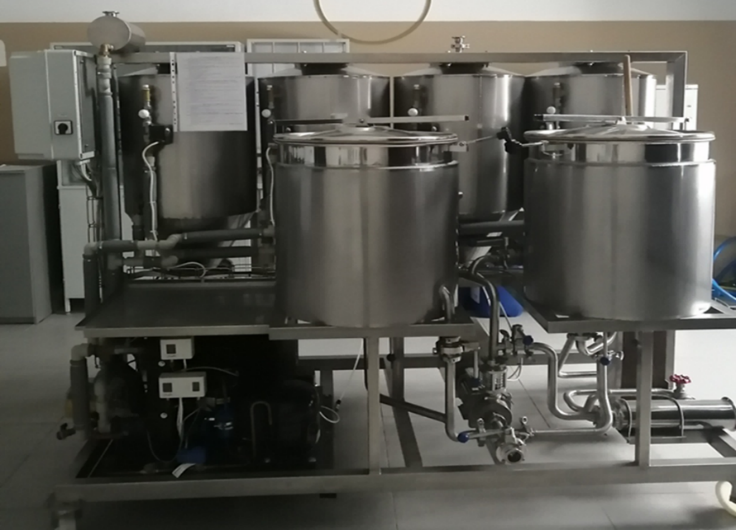
\includegraphics[width=0.8\textwidth]{media/pish3/image4}
	\caption*{}
\end{figure}


{\bfseries 1 - сурет. NANО BREWERY TYPE 50 L4 шағын сыра зауыты}

{\bfseries Нәтижелер және талқылау.} Бидай уытын өндіру үшін көктемгі және
қысқы егістік бидай сұрыптары іріктелінді. "Тәуелсіздік-20" сұрыпы
крахмалдың жоғары мөлшерімен сипатталса, барлық сұрыптарда ақуыздың
мөлшері сыра өндіруге рұқсат етілген шектерден (8-12\%) сәл асып түсті.
Суға сезімталдық көрсеткіші оңтайлы ауқымда болған бидай сұрыптары
ақуызы жоғары еритімділікке, жоғары ашытқыш қуатына және жоғары
диастатикалық қуатқа ие уыт алуға мүмкіндік береді {[}Narciss{]}.

Ұсынылған бидай сұрыптарынан уыт өндіру сыра өндіруге арналған уыттың
классикалық технологиясы бойынша белгілі параметрлерді сақтай отырып
жүргізілді. Уыт дайындау 15°С температурада 4,5 тәулік бойы жүргізілді.
Ұрықтандыру кезінде дәндер күніне 2 рет араластырылып, су бүркілді.
Ұрықтандыруды бақылау көзбен жүргізілді. Күн сайын ылғалдылықты
тексеріп, суғарып, араластырып отырды. Дән ұрығы дән ұзындығының
2/3-3/4-іне жеткенде ұрықтандыруды тоқтатты. Кептіру Binder FD-23
вакуумдық кептіргіш шкафында жүргізілді. Кептіру температурасы 45°С-тан
бастап 14 сағат ішінде біртіндеп 80°С-қа дейін көтерілді. Нәтижесінде
келесі сипаттамаларға ие бидай уыттары алынды (3-кесте).

{\bfseries 3-кесте - Бидай уытының физика-химиялық көрсеткіштері}

% \begin{longtable}[]{@{}
%   >{\raggedright\arraybackslash}p{(\columnwidth - 6\tabcolsep) * \real{0.3156}}
%   >{\raggedright\arraybackslash}p{(\columnwidth - 6\tabcolsep) * \real{0.2239}}
%   >{\raggedright\arraybackslash}p{(\columnwidth - 6\tabcolsep) * \real{0.2368}}
%   >{\raggedright\arraybackslash}p{(\columnwidth - 6\tabcolsep) * \real{0.2237}}@{}}
% \toprule\noalign{}
% \begin{minipage}[b]{\linewidth}\raggedright
% Көрсеткіш
% \end{minipage} & \begin{minipage}[b]{\linewidth}\raggedright
% Ертіс-7 (жаздық дақыл)
% \end{minipage} & \begin{minipage}[b]{\linewidth}\raggedright
% Тәуелсіздік-20 (жаздық дақыл)
% \end{minipage} & \begin{minipage}[b]{\linewidth}\raggedright
% Матай (қыстық дақыл)
% \end{minipage} \\
% \midrule\noalign{}
% \endhead
% \bottomrule\noalign{}
% \endlastfoot
% Ылғалдың массалық үлесі, \% & 4,82±0,3 & 4,92±0,3 & 5,6±0,4 \\
% ҚЗ-ға экстрактивті заттардың массалық үлесі, \% & 74,88±0,2 & 82,3±0,2 &
% 72,3±0,2 \\
% ҚЗ бойынша уыттағы ақуыз заттардың массалық үлесі, \% & 12,90±0,3 &
% 14,2±0,4 & 14,8±0,4 \\
% Кольбах саны, \% & 52,3±1,9 & 42,6±1,8 & 43,4±1,8 \\
% Амин азот мөлшері, 100 г сығындыға мг & 119,80±6,0 & 180,8±5,0 &
% 291,0±4,0 \\
% Диастатикалық күш, бірлік°WK & 423,9±10,7 & 351,3±16,1 & 450,4±13,3 \\
% Қанттандыру уақыты, мин & 13,0±1,0 & 14,0±1,0 & 14,0±1,0 \\
% Сусланың тұтқырлығы, мПа•с & 1,5±0,1 & 1,6±0,1 & 1,5±0, \\
% сусланың рН & 5,68±0,1 & 6,1±0,1 & 6,2±0,1 \\
% Титрленетін қышқылдық & 1,5±0,1 & 1,1±0,1 & 1,5±0,1 \\
% \end{longtable}

Бидай уытының тұтқырлығы және түсі жоғары болды, ақуыздың мөлшері МЕМСТ
29294 бойынша қалыпты 12,2\%-дан асып түсті. "Ертіс-7" бидайынан алынған
уыттың экстракттік шығымы төмен (шамамен 75\%) болды. Ақуызы жоғары
(14-18\%) бидайдан жоғары экстрактті уыт алу мүмкін емес. Уыт жоғары
диастатикалық қуаттылық пен стандартты қанттандыру уақытын көрсетті.
Төмендейтін температураларда жоғары диастатикалық қуаттылық "Ертіс-7"
және "Тәуелсіздік-20" бидайларын уыттау кезінде байқалды. Осы уыттан
дайындалған суслоның тұтқырлығы жоғары болған жоқ. "Ертіс-7" бидайы үшін
төмендейтін температуралардың әсері "Тәуелсіздік-20" сұрыпындай болмады.
Мүмкін, бидай дәнін бағалау үшін уыттаудың белгілі бір технологиясын
қолдануға арналған қосымша параметрлер қажет.

Алынған уыттар негізінде бидай сырасының рецептурасы есептелді және оны
өндіру технологиясы әзірленді. МЕМСТ 31711 бойынша бидай сырасын өндіру
үшін кем дегенде 50\% бидай уытын қолдану қажет. Бидай сырасын өндіру
үшін мынадай ингредиенттер пайдаланылды: Арпа уыты -- 40\% (ақшыл
негізгі -- 30-40\%, карамельді 150 -- 10\%); Бидай уыты - 50-60\%; Неміс
гранулалы хмелі «El Dorado» (α-қышқылы 12,8\%) және «Cascade» (α-қышқылы
4,2\%); Құлмақтың қосылу нормасы: 1 литр ыстық суслоға 0,041 г
α-қышқылы; Сұйық жоғарғы ашытқы WB-06 (50 мл); Гидромодуль 1/4 құрады.
3-кестеде Қазақстандық бидай уыттарынан жасалған бидай сырасының
әзірленген рецептуралары көрсетілген: Рецептура 1: "Ертіс-7" бидай уыты
(60\%); Рецептура 2: "Тәуелсіздік-20" бидай уыты (60\%); Рецептура 3:
"Матай" бидай уыты (50\%).

{\bfseries 4-кесте. Қазақстандық бидай уыттарынан жасалған бидай сырасының
рецептуралары}

% \begin{longtable}[]{@{}
%   >{\raggedright\arraybackslash}p{(\columnwidth - 8\tabcolsep) * \real{0.3475}}
%   >{\raggedright\arraybackslash}p{(\columnwidth - 8\tabcolsep) * \real{0.2130}}
%   >{\raggedright\arraybackslash}p{(\columnwidth - 8\tabcolsep) * \real{0.1365}}
%   >{\raggedright\arraybackslash}p{(\columnwidth - 8\tabcolsep) * \real{0.1665}}
%   >{\raggedright\arraybackslash}p{(\columnwidth - 8\tabcolsep) * \real{0.1365}}@{}}
% \toprule\noalign{}
% \begin{minipage}[b]{\linewidth}\raggedright
% Компонент атауы
% \end{minipage} & \begin{minipage}[b]{\linewidth}\raggedright
% Бақылау
% \end{minipage} & \begin{minipage}[b]{\linewidth}\raggedright
% Рецептура
% 
% 1
% \end{minipage} & \begin{minipage}[b]{\linewidth}\raggedright
% Рецептура
% 
% 2
% \end{minipage} & \begin{minipage}[b]{\linewidth}\raggedright
% Рецептура
% 
% 3
% \end{minipage} \\
% \midrule\noalign{}
% \endhead
% \bottomrule\noalign{}
% \endlastfoot
% Ақшыл арпа уыты, кг & 30 \%-дан
% 
% 50 \%-ға дейін & 80 & 80 & 90 \\
% Ақшыл бидай уыты, кг & 50 \%-дан кем емес & 110 & 110 & 100 \\
% Карамельді уыт -150, кг & 0-ден
% 
% 20 \%-ға дейін & 10 & 10 & 10 \\
% Құлмақ El Dorado (α=12,8 \%), кг & 2,72/α;
% 
% 12 IBU & 0,225 & 0,225 & 0,225 \\
% Құлмақ Cascade (α=4,8 \%),
% 
% кг & 0,92/α;
% 
% 12 IBU & 0,230 & 0,230 & 0,230 \\
% Ашытқы WB-06, кг & 10 млн.
% 
% жасуша/мл & 0,5 & 0,5 & 0,5 \\
% \end{longtable}

Ұсынылған рецептуралар негізінде бидай уытын өндірудің негізгі
технологиялық режимдері таңдалды және оларға негізделген сыра өндірудің
технологиялық схемасы әзірленді (2-сурет). Түсі 150 EBC болатын
карамельді уыт-150 сыраның түсін және хош иісін күшейту, сонымен қатар
оған қанық түс пен дәм беру үшін қолданылды.

\begin{figure}[H]
	\centering
	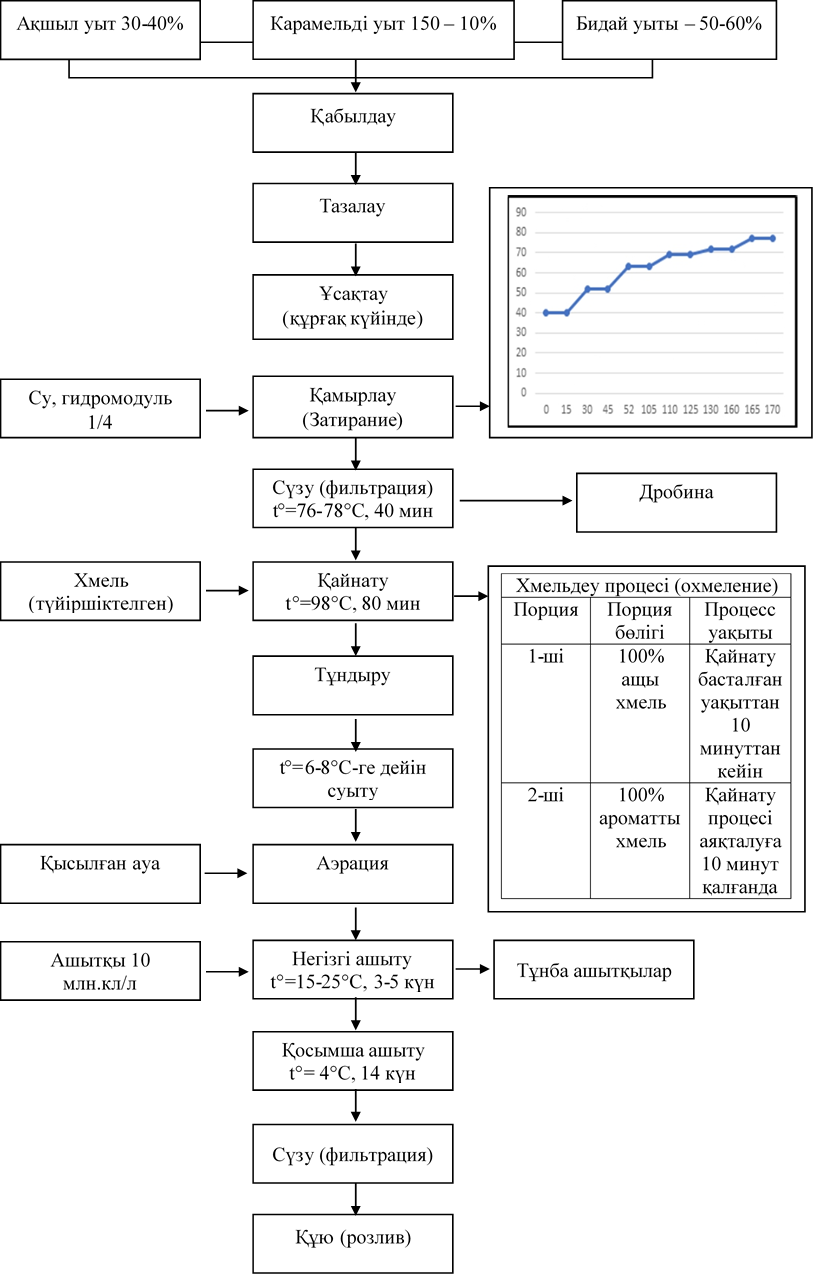
\includegraphics[width=0.8\textwidth]{media/pish3/image5}
	\caption*{}
\end{figure}


{\bfseries 2- сурет. Бидай сырасының өндірісінің технологиялық сұлбасы}

Сыра суслосын алудың негізгі процестерінің бірі -- қамырлау(затирание).
Қамырлау ұсақталған дән өнімдерін сумен араластыру арқылы басталады. Дән
қоспасы жоспарлы бастапқы экстрактілік сусло мөлшеріне байланысты
есептеледі. Жеңіл сыралар үшін (спирт мөлшері аз) бастапқы экстрактілік
сусло 8\% (ақшыл сыра), 11\% (қоңыр және бидай сырасы) құрайды. Күшті
сыралар үшін бастапқы экстрактілік сусло 22\% дейін жетеді (МЕМСТ
31711).

Бидай уытынан сусло алу үшін 40°С цитолиттік температуралық үзілісті
қолдану ұсынылады. Қамырлау инфузиялық әдіспен жүргізілді.

Қамырлау келесі жағдайларда жүргізілді: 40°С - бидай уыты бар қоспалар
үшін цитолиттік үзіліс, 52°С - ақуыздық үзіліс, 62°С - мальтоза үзілісі,
72°С - қанттандыру үзілісі. Қоспаның pH 5.9. Үзілістердің ұзақтығы 15-60
минутты құрады, қыздыру жылдамдығы 1°С/мин.

Қоспа құрамы мен температуралық үзілістердің әсерін зерттеуден бұрын,
арпа және бидай уыттары сыра суслосының сапасына әсер ететін негізгі
параметрлер бойынша талданды. Қанттандырылған қоспа 76-77°С
температурада дробинадан бөлінді. Бірінші суслоның экстрактілігі 16,4\%
құрады, алынған сусло қоңыр қанық түске ие болды. Дробина 77-78°С ыстық
сумен жуылды және онымен негізгі сусло 14,5\% экстрактілікке дейін
сейілтті. Құлмақпен сусло қайнатылған кезде, судың булануына байланысты,
суслоның экстрактілігі 12\%-ға дейін көтерілді. Алынған сусло құлмақпен
80 минут қайнатылды, құлмақ бірдей екі порциямен қосылды: сусло
қайнағаннан кейін 10 минут өткен соң және қайнату аяқталғанға 10 минут
қалғанда. Суслодағы құрғак заттардың бастапқы мөлшері 12\% құрады. Сусло
суытылғаннан кейін, сұйық ашытқылар қосылды. Негізгі ашыту 19°С
температурада жүргізілді. Нақты ашытқыш қуаты 60\% (құрғак заттардың
мөлшері 4,8\%) 3-5 күнде қол жеткізілді. Қосымша ашыту 4°С температурада
2 апта бойы жүргізілді.

Келесі зерттеулер сериясы әзірленген сусындардың физика-химиялық және
органолептикалық сипаттамаларын талдаудан тұрды. 5-кестеде әзірленген
сыраның физика-химиялық сапа көрсеткіштері көрсетілген.

{\bfseries 5-кесте. Өндірілген сыра сапасының физика-химиялық
көрсеткіштері}

% \begin{longtable}[]{@{}
%   >{\raggedright\arraybackslash}p{(\columnwidth - 6\tabcolsep) * \real{0.2864}}
%   >{\raggedright\arraybackslash}p{(\columnwidth - 6\tabcolsep) * \real{0.2515}}
%   >{\raggedright\arraybackslash}p{(\columnwidth - 6\tabcolsep) * \real{0.2439}}
%   >{\raggedright\arraybackslash}p{(\columnwidth - 6\tabcolsep) * \real{0.2182}}@{}}
% \toprule\noalign{}
% \begin{minipage}[b]{\linewidth}\raggedright
% Көрсеткіш
% \end{minipage} & \begin{minipage}[b]{\linewidth}\raggedright
% Үлгі 1
% \end{minipage} & \begin{minipage}[b]{\linewidth}\raggedright
% Үлгі 2
% \end{minipage} & \begin{minipage}[b]{\linewidth}\raggedright
% Үлгі 3
% \end{minipage} \\
% \midrule\noalign{}
% \endhead
% \bottomrule\noalign{}
% \endlastfoot
% Бастапқы сусланың экстрактивтілігі, \% & 10 & 12 & 12 \\
% Алкоголь құрамы, \% об. & 4,2 & 4,3 & 4,3 \\
% Ашытудың нақты дәрежесі, \% & 68 & 70 & 72 \\
% рН & 4,1 & 4,2 & 4,3 \\
% Түс көрсеткіші, EBC & 10 & 16 & 12 \\
% \end{longtable}

Тәжірибелік үлгілердің физика-химиялық параметрлері классикалық ақшыл
сыра үшін қалыпты диапазонда болды. 2-үлгіге арналған түс индексі орташа
мәннен жоғары, бірақ ақшыл сыра үшін қолайлы диапазонда, бұл негізі оның
ерекше химиялық құрамына байланысты.

3-суретте әзірленген сыра сұрыптарының фотосуреттері көрсетілген.

Органолептикалық көрсеткіштері бойынша 1, 2 үлгілерде көбік тұрақтылығы
төмендеген, бұл факт езгілеу процесінде ақуыздың толық ерімейтіндігімен
түсіндіріледі, ал 3-үлгі құрамында көмірқышқыл газының мөлшері орташа
болған кезде органолептикалық көрсеткіштері жақсы болды.

\begin{figure}[H]
	\centering
	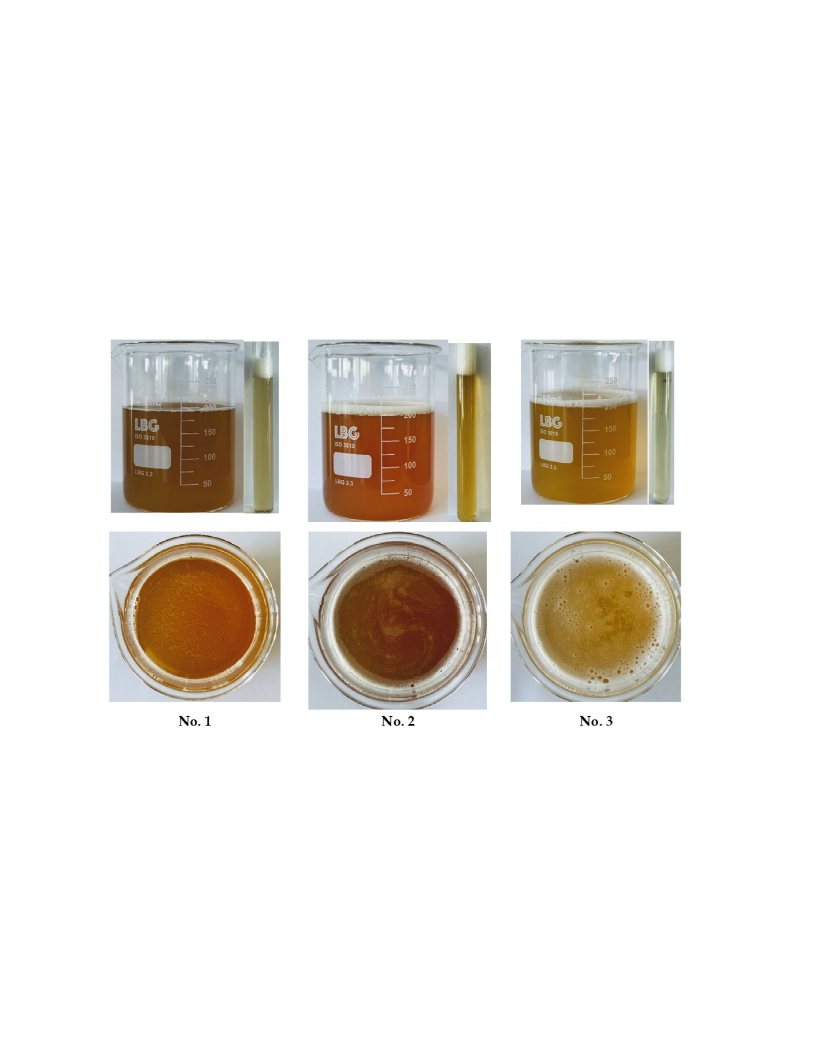
\includegraphics[width=0.8\textwidth]{media/pish3/image6}
	\caption*{}
\end{figure}


{\bfseries 3-сурет. Сыра үлгілерінің суреттері}

\emph{(№1 - "Ертіс-7" бидай сұрыпынан алынған уыт қосылған сыра (60\%);
№2 - "Тәуелсіздік-20" бидай сұрыпынан алынған уыт қосылған сыра (60\%);
№3 - "Матай" бидай сұрыпынан алынған уыт қосылған сыра (50}\%)).

{\bfseries Қорытынды.} Ақшыл сыра өндіруге арналған отандық селекциялы
бидайдың дәнді дақылдары негізделіп, іріктелді. Қазақстан
Республикасында аудандастырылған бидайдың 5 сұрыптарынан сыра өндірісі
үшін физика-химиялық көрсеткіштері жақсартылған (крахмал мөлшері
72-82\%, ақуыз 12-14\%) «Ертіс», «Матай», «Тәуелсіздік-20». Сұрыптары
зерттеуге іріктелді.

Құйылатын езбе мөлшері және ысқылау режимдері таңдалды. Арнайы химиялық
құрамын ескере отырып, сыра өндіруге арналған рецепттер әзірленді.

Отандық селекциялы бидай дәнін пайдаланып, сыра өндірудің технологиялық
картасы мен технологиялық сұлбасы әзірленді және олардың сапа
көрсеткіштері зерттелді. Эксперименттік сыра үлгілері сипаттамалары
бойынша классикалық ақшыл сыраға сәйкес келетіні дәлелденді.

{\bfseries Литература}

1. Агафонов В.П., Оболенский Н.В. Диагностика и перспективы развития
российского рынка пива // Прикладные экономические исследования.- 2014.
- № 3. - с.20-25.

2. Baigaziyeva G.I., Kekibaeva A.K., Akhmetzhanova A.K., Kerimbayeva
A.A. Prospects for the use of new yeast strains in non-alcoholic beer
production//The Journal of Almaty Technological University.
-2024.-T.146(4) -P.86-96-85.
\href{https://doi.org/10.48184/2304-568X-2024-4-78-86}{DOI
10.48184/2304-568X-2024-4-78-86}

3.Curtis S. Cereals in Brewing and Destilling. Brew. Distill. Int.
2011;7:8--9.~{[}Google Scholar{]}

ISSN (Print): 1753-2086.
URL:~\href{http://www.ibd.org.uk/}{http://www.ibd.org.uk}. CABI Record
Number: 20113177395

4. Шаболкина Е. Н., Мясникова М. Г., Мальчиков П. Н., Пронович Л. В.
Возможности использования зерна твёрдой пшеницы в хлебопекарной
промышленности // Зернобобовые и крупяные культуры. -2016.- №4.- C..
26-31.

5. Ростовская М.Ф., Загария С.Ю., Алябьев Б.А., Клыков А.Г. Пивоваренный
солод из сортов пшеницы, возделываемых в Приморском крае //Пиво и
напитки. -2009. -№ 4. -- с. 36-38.

6. Белокурова Е. С. Повышение конкурентоспособности отечественного
пивоваренного ячменя // Пиво и напитки. -2008. -№ 3.- c. 8-9.

7. Киселева Т.Ф., Помозова В.А., Миллер Ю.Ю., Верещагин А.Л.
Совершенствование технологии пшеничного солода // Пиво и напитки. 2017.
№ 5.- c. 10-14-51.

8. Ростовская М.Ф., Извекова А.Н., Извекова Н.Н. Влияние параметров
солодоращения на качество пшеничного солода // Пиво и напитки. -2014.
-№4.- С.54-56.

9. Киселева Т.Ф., Гребенникова Ю.В. Использование соевого и пшеничного
солодов в производстве напитков брожения // Пищевая промышленность.-
2019. - № 5.- С. 10-14

10. Гоенко В.А., Назаренко Т.А. Исследование технологических и
потребительских свойств некондиционного зерна пшеницы // Проблемы Науки.
2019.

URL:https://cyberleninka.ru/article/n/issledovanie-tehnologicheskih-i-potrebitelskih-svoystv-nekonditsionnogo-zerna-pshenitsy

11.Троценко А. С., Танашкина Т. В., Корчагин В. П., Клыков А. Г.
Проблемы и перспективы использования гречихи в пищевой биотехнологии //
Вестник ТГЭУ.- 2010.-№ 2.-С.104-116

12. Нарцисс Л. Технология солодоращения / Л. Нарцисс - пер. с нем. под
общей ред. Г. А. Ермолаевой, Е. Ф. Шапенко. -- СПб.: Профессия, 2007. -
565 c. ISBN 5-939113-118-2

13. Бак В. Практическое руководство по технологии пивоварения / В. Бак.
-- 2-е изд., пер. с нем., науч. ред. перевода Г. Ермолаева. - Бремен,
2013. - 427 с.

14. Depraetere S., Delvaux F., Coghe S.,. Delvaux F.R. A. Wheat variety
and barley malt properties: influence on haze intensity and foam
stability of wheat beer. / // Journal of the institute of brewing.
-2004. -110 (3). -P.200-2006. DOI 10.1002/j.2050-0416.2004.tb00203.x

15. \href{https://onlinelibrary.wiley.com/authored-by/Jin/Yuhong}{Yuhong
Jin},~\href{https://onlinelibrary.wiley.com/authored-by/Zhang/Kaili}{Kaili
Zhang},~\href{https://onlinelibrary.wiley.com/authored-by/Du/Jinhua}{Jinhua
Du} Effects of wheat protein content on endosperm composites and malt
quality//Journal of the institute of brewing.-2008.-114 (4).- 289-293.

\href{https://doi.org/10.1002/j.2050-0416.2008.tb00771.x}{DOI
10.1002/j.2050-0416.2008.tb00771.x}

{\bfseries References}

1. Agafonov V.P., Obolenskij N.V. Diagnostika i perspektivy razvitija
rossijskogo rynka piva // Prikladnye jekonomicheskie issledovanija.-
2014. - № 3. - s.20-25.

2. Baigaziyeva G.I., Kekibaeva A.K., Akhmetzhanova A.K., Kerimbayeva
A.A. Prospects for the use of new yeast strains in non-alcoholic beer
production//The Journal of Almaty Technological University.
-2024.-T.146(4) -P.86-96-85.
\href{https://doi.org/10.48184/2304-568X-2024-4-78-86}{DOI
10.48184/2304-568X-2024-4-78-86}

3.Curtis S. Cereals in Brewing and Destilling. Brew. Distill. Int.
2011;7:8--9.~{[}Google Scholar{]}

ISSN (Print): 1753-2086.
URL:~\href{http://www.ibd.org.uk/}{http://www.ibd.org.uk}. CABI Record
Number: 20113177395

4. Shabolkina E. N., Mjasnikova M. G., Mal' chikov P. N.,
Pronovich L. V. Vozmozhnosti ispol' zovanija zerna
tvjordoj pshenicy v hlebopekarnoj promyshlennosti // Zernobobovye i
krupjanye kul' tury. -2016.- №4.- C.. 26-31.

5. Rostovskaja M.F., Zagarija S.Ju., Aljab' ev B.A.,
Klykov A.G. Pivovarennyj solod iz sortov pshenicy, vozdelyvaemyh v
Primorskom krae //Pivo i napitki. -2009. -№ 4. -- s. 36-38.

6. Belokurova E. S. Povyshenie konkurentosposobnosti otechestvennogo
pivovarennogo jachmenja // Pivo i napitki. -2008. -№ 3.- c. 8-9.

7. Kiseleva T.F., Pomozova V.A., Miller Ju.Ju., Vereshhagin A.L.
Sovershenstvovanie tehnologii pshenichnogo soloda // Pivo i napitki.
2017. № 5.- c. 10-14-51.

8. Rostovskaja M.F., Izvekova A.N., Izvekova N.N. Vlijanie parametrov
solodorashhenija na kachestvo pshenichnogo soloda // Pivo i napitki.
-2014. -№4.- S.54-56.

9. Kiseleva T.F., Grebennikova Ju.V. Ispol' zovanie
soevogo i pshenichnogo solodov v proizvodstve napitkov brozhenija //
Pishhevaja promyshlennost'.- 2019. - № 5.- S. 10-14

10. Goenko V.A., Nazarenko T.A. Issledovanie tehnologicheskih i
potrebitel' skih svojstv nekondicionnogo zerna pshenicy
// Problemy Nauki. 2019.

URL:https://cyberleninka.ru/article/n/issledovanie-tehnologicheskih-i-potrebitelskih-svoystv-nekonditsionnogo-zerna-pshenitsy

11.Trocenko A. S., Tanashkina T. V., Korchagin V. P., Klykov A. G.
Problemy i perspektivy ispol' zovanija grechihi v
pishhevoj biotehnologii // Vestnik TGJeU.- 2010.-№ 2.-S.104-116

12. Narciss L. Tehnologija solodorashhenija / L. Narciss - per. s nem.
pod obshhej red. G. A. Ermolaevoj, E. F. Shapenko. -- SPb.: Professija,
2007. - 565 c. ISBN 5-939113-118-2

13. Bak V. Prakticheskoe rukovodstvo po tehnologii pivovarenija / V.
Bak. -- 2-e izd., per. s nem., nauch. red. perevoda G. Ermolaeva. -
Bremen, 2013. - 427 s.

14. Depraetere S., Delvaux F., Coghe S.,. Delvaux F.R. A. Wheat variety
and barley malt properties: influence on haze intensity and foam
stability of wheat beer. / // Journal of the institute of brewing.
-2004. -110 (3). -P.200-2006. DOI 10.1002/j.2050-0416.2004.tb00203.x

15. \href{https://onlinelibrary.wiley.com/authored-by/Jin/Yuhong}{Yuhong
Jin},~\href{https://onlinelibrary.wiley.com/authored-by/Zhang/Kaili}{Kaili
Zhang},~\href{https://onlinelibrary.wiley.com/authored-by/Du/Jinhua}{Jinhua
Du} Effects of wheat protein content on endosperm composites and malt
quality//Journal of the institute of brewing.-2008.-114 (4).- 289-293.

\href{https://doi.org/10.1002/j.2050-0416.2008.tb00771.x}{DOI
10.1002/j.2050-0416.2008.tb00771.x}

\emph{{\bfseries Сведения об авторах}}

Бакытжан Д.Н. - докторант, Алматинский Технологический Университет, г.
Алматы, Казахстан, e-mail:
\href{mailto:didar_99_kz@mail.ru}{\nolinkurl{didar\_99\_kz@mail.ru}};

Аскарбеков Э.Б. Доктор PhD, ассоц.профессор, Казахский университет
технологий и бизнеса, Астана, Казахстан, e-mail Erik\_ab82@mail.ru;

Байгазиева Г.И. - к.б.н., и.о профессора, Алматинский Технологический
Университет, г. Алматы, Казахстан, e-mail: gulgaishailias@mail.ru;

Кекибаев А.К. - к.б.н., ассоц. профессор, Алматинский Технологический
Университет, г. Алматы, Казахстан, e-mail: anara\_06061983@mail.ru

\emph{{\bfseries Information about the authors}}

Bakytzhan D.N.-Doctoral student, Almaty Technological University,
Almaty, Kazakhstan, e-mail: didar\_99\_kz@mail.ru ;

Askarbekov E.B. PhD, Assoc.Professor, Kazakh University of Technology
and Business, Astana, Kazakhstan, e-mail Erik\_ab82@mail.ru;

Baigazieva G.I. - Candidate of Biological Sciences, Acting Professor,
Almaty Technological University, Almaty, Kazakhstan, e-mail:
gulgaishailias@mail.ru;

Kekibaev A.K. - Candidate of Biological Sciences, Associate Professor,
Almaty Technological University, Almaty, Kazakhstan, e-mail:
anara\_06061983@mail.ru

\begin{longtable}[]{@{}
  >{\raggedright\arraybackslash}p{(\columnwidth - 0\tabcolsep) * \real{1.0000}}@{}}
\toprule\noalign{}
\begin{minipage}[b]{\linewidth}\raggedright